\documentclass[12pt, a4paper, oneside]{book}%,twocolumn %pour deux colonnes mais il faut changer dautre choses aussipour que ca rend bien et avec deux colonnes on reduit notre rappport de 33 pages a 20 pages 
\usepackage[T1]{fontenc}
\usepackage[utf8]{inputenc}

\usepackage{parskip}  %pour paragraphs
\setlength{\parindent}{15pt}
\usepackage{fourier}
\usepackage{afterpage}
\usepackage[cmex10]{amsmath}
\usepackage{amssymb}
\usepackage[pdftex]{graphicx}
\usepackage{epstopdf}
\epstopdfsetup{update}
\usepackage{fancyhdr}
\usepackage[twoside, margin=2.5cm, bindingoffset=0.0cm]{geometry}
\usepackage{url}
\usepackage{siunitx}
\usepackage{float}

\usepackage[caption = false]{subfig}
\usepackage{alphalph}
\renewcommand*{\thesubfigure}{%
\alphalph{\value{subfigure}}%
}

\usepackage{amsthm}
\theoremstyle{definition}
\newtheorem{definition}{Definition}[section]

\theoremstyle{remark}
\newtheorem*{remark}{Remark}

\newtheorem{theorem}{Theorem}[section]
\newtheorem{corollary}{Corollary}[theorem]
\newtheorem{lemma}[theorem]{Lemme}

\usepackage{algorithm}
\usepackage{algpseudocode}
\renewcommand{\algorithmicforall}{\textbf{for each}}

\usepackage{tabularx}

%\sisetup{detect-all,input-product=*}%
% \usepackage[labelformat=simple]{subcaption}
% \captionsetup{font={footnotesize,sf},skip=2pt}

% \usepackage[%backend=biber,
% style = ieee,
% sorting=none
% ]{biblatex} %,bibstyle=ieeehttps://www.overleaf.com/project/624dc5f129c1767e8bb8de67
% \addbibresource{biblio.bib}
% \renewbibmacro*{date}{%
%   \iffieldundef{year}
%     {\bibstring{nodate}}
%     {\printdate}
% }
%\usepackage{svg}
\usepackage[inkscapeformat=png]{svg}
\usepackage{tikz}
\usetikzlibrary{matrix,calc}
\DeclareMathOperator{\sech}{sech}

\usepackage[%backend=biber,
style = ieee,
sorting=none,
% style=authoryear-icomp,
% maxbibnames=9,
% maxcitenames=1,
]{biblatex} %,bibstyle=ieeehttps://www.overleaf.com/project/624dc5f129c1767e8bb8de67

\addbibresource{biblio.bib}
\renewbibmacro*{date}{%
  \iffieldundef{year}
    {\bibstring{nodate}}
    {\printdate}
}

\usepackage{hyperref} %For hyperlinks 
\hypersetup{pdfborder=0 0 0}
\usepackage[french]{babel} %language correction
\usepackage{romannum}
\usepackage{perpage}
\usepackage{csquotes}
\MakePerPage{footnote}

\usepackage{indentfirst}

%%%%%%%%%%%%%%%%%%%%%%%%%%%%%%
%For glossaries 
%%%%%%%%%%%%%%%%%%%%%%%%%%%%%%

%\usepackage{glossaries}
%\usepackage{glossary-mcols}
%\makeglossaries
%\renewcommand*{\glspostdescription}{} % Removes dots at the end of each entry.

%\DeclareGraphicsRule{.wmf}{bmp}{}{}% declare WMF filename extension
\graphicspath{{Figures/}}
\usepackage{chngcntr}
\counterwithin{figure}{section} %changer a subsection 

%%%%%%%%%%%%%%%%%%%%%%%%%%%%%%
%POUR LES CODES
%%%%%%%%%%%%%%%%%%%%%%%%%%%%%
%https://www.overleaf.com/learn/latex/Code_listing
\usepackage{listings}
\usepackage{xcolor}
\usepackage[section]{placeins}
\usepackage{enumitem}
\usepackage{accsupp}

\newcommand{\noncopynumber}[1]{%
    \BeginAccSupp{method=escape,ActualText={}}%
    #1%
    \EndAccSupp{}%
}

\definecolor{codegreen}{rgb}{0,0.6,0}
\definecolor{codegray}{rgb}{0.5,0.5,0.5}
\definecolor{codepurple}{rgb}{0.58,0,0.82}
\definecolor{backcolour}{rgb}{0.95,0.95,0.92}

\lstdefinestyle{mystyle}{
    backgroundcolor=\color{backcolour},   
    commentstyle=\color{codegreen},
    keywordstyle=\color{magenta},
    numberstyle=\tiny\color{codegray},
    stringstyle=\color{codepurple},
    basicstyle=\ttfamily\footnotesize,
    breakatwhitespace=false,         
    breaklines=true,                 
    captionpos=b,                    
    keepspaces=true,                 
    numbers = left,
    numberstyle=\tiny\noncopynumber,
    numbersep=5pt,                  
    showspaces=false,                
    showstringspaces=false,
    showtabs=false,                  
    tabsize=2
}
\lstset{style=mystyle}

%\begin{lstlisting}[language=Python, caption=Python example]
%VOtre Code
%\end{lstlisting}
%\lstinputlisting[language=Octave]{BitXorMatrix.m}%pour importer directement dun fichier

% \usepackage{physics}
\usepackage{booktabs}
% \usepackage{subfig}

%%%%%%%%%%%%%%%%%%%%%%%%%%%%%%%%%%%%%%%%%%%%%%%%%%
%Des Raccourcies
%%%%%%%%%%%%%%%%%%%%%%%%%%%%%%%%%%%%%%%%%%%%%%%%%%
\newcommand{\comment}[1]{}%pour faire des comentaires a plusueures lignes 
\usepackage{xstring}
\newcommand{\AncaBelme}{Anca Belme}
\newcommand{\AncaBELME}{Anca BELME}
\newcommand{\ijlrd}{Institut Jean le Rond $\partial ' \textrm{Alembert}$ \space}
\newcommand{\JeanCamilleChassaing}{Jean-Camille Chassaing}
\newcommand{\JeanCamilleCHASSAING}{Jean-Camille CHASSAING}
\newcommand{\RemyCornaggia}{Rémi Cornaggia}
\usepackage{bm}%\newcommand{\bm}[1]{\mathbf{#1}}

\fancypagestyle{firstpage}{
\setlength{\headheight}{60pt}
\fancyhead[L]{
\includegraphics[height=0.1\textwidth]{SORBONNE_FAC_SCIENCES_DEF_CMJN.png}
              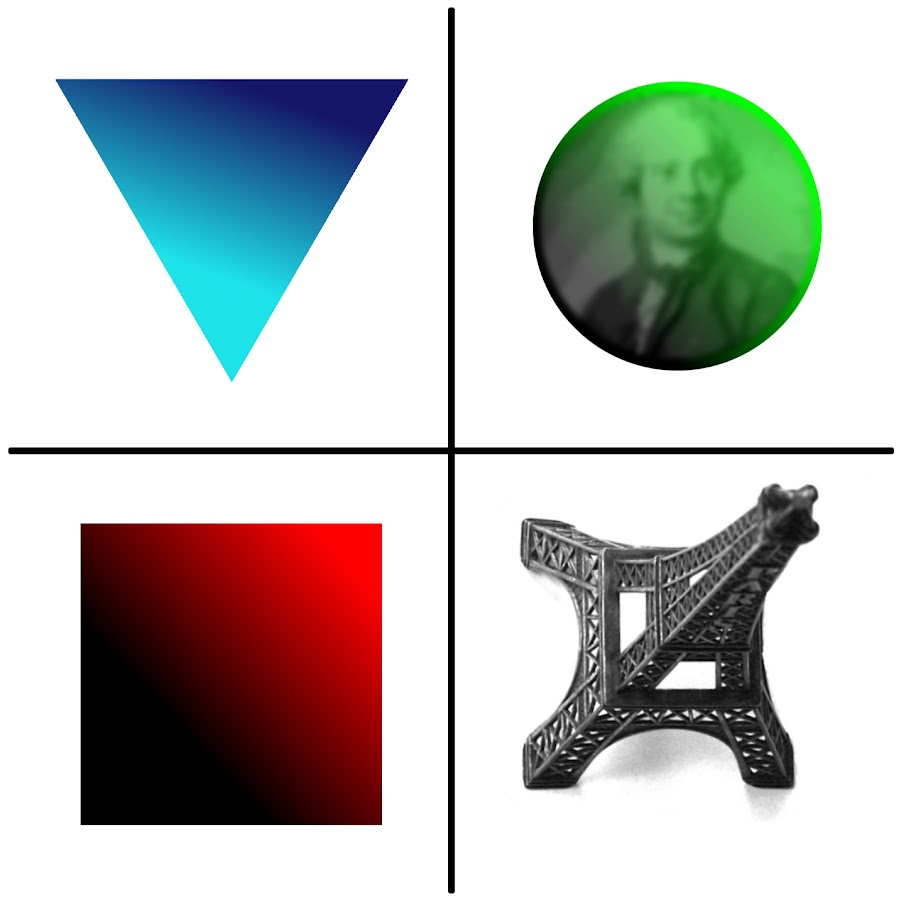
\includegraphics[height=0.1\textwidth]{Figures/logo_minimal_institut_jean_le_rond_dalembert.jpg}}
\fancyhead[R]{{\Large{ 3\up{e} }}}%semestre de l'année universitaire 2021-2022\\L1 CMI Mécanique}}}
\fancyfoot{}}

%\setlength{\parindent}{0pt}
\setlength{\parskip}{2ex plus 1ex minus 1ex}

\newcommand{\HeaderDeReapport}{Rapport de Stage}% Erdi ÇAN}
\newcommand\blankpage{%
    \null
    \thispagestyle{empty}%
    \addtocounter{page}{-1}%
    \newpage
}
  
\usepackage{atbegshi,picture}
\usepackage{lipsum}


\AtBeginShipoutNext{\AtBeginShipoutUpperLeft{%
  \put(\dimexpr\paperwidth-1cm\relax,-3cm){\makebox[0pt][r]{\Large Cursus de Master en Ingénierie  $3^{\textrm{e}}$ année }}%\framebox{Copyright DTV}}}%
}}


\begin{document}

% TODO 
% \begin{itemize}
%     \item turbulence le developper avec les statistiques de plus grande ordre unpeut plus de detail et choses fait 
%     \item Les modeles et les developper 
%     \item annexe 
%     \begin{itemize}s
%         \item autre choses fait 
%         \item derniere semaine coup doeil sur le programme de ptv 
%         \item simultaion sph avec dualsphysics
%         \begin{itemize}
%             \item pourquoi ca a pas marche 
%             \item comparisons avec des resultats mais il ya pas de beses de donnees testable cest de meme raison que on nest pas alle plus loin avec la simulation avec le manque de donnees et deja que on a des problemes avec 74 points. 
%         \end{itemize}
%     \end{itemize}
%     \item conclusion
% \end{itemize}
% \newpage


\vspace{250pt}
\title{
    \normalsize\bfseries{\HeaderDeReapport}\\
    \vspace{10pt}
    \Large\bfseries TODO
    %\vspace{10pt}
    %\textit{Intermediate Report}}
}

\author{Erdi ÇAN\\Samy DUMONT\\Encadré par \AncaBELME} %\\ Enseignant référent : \JeanCamilleCHASSAING}
\date{10 septembre 2023}

\maketitle

% TODO put figures on the title page 
\tikz[remember picture, overlay] 
\node[shift={(1cm,-1cm)}] at (current page.north west) %
[anchor=north west] %
{
\includegraphics[height = 2cm]{Figures/SORBONNE_FAC_SCIENCES_DEF_CMJN.png}};

\tikz[remember picture, overlay] %
\node[shift={(6.5cm,-1cm)}] at (current page.north west) %
[anchor=north west] %
{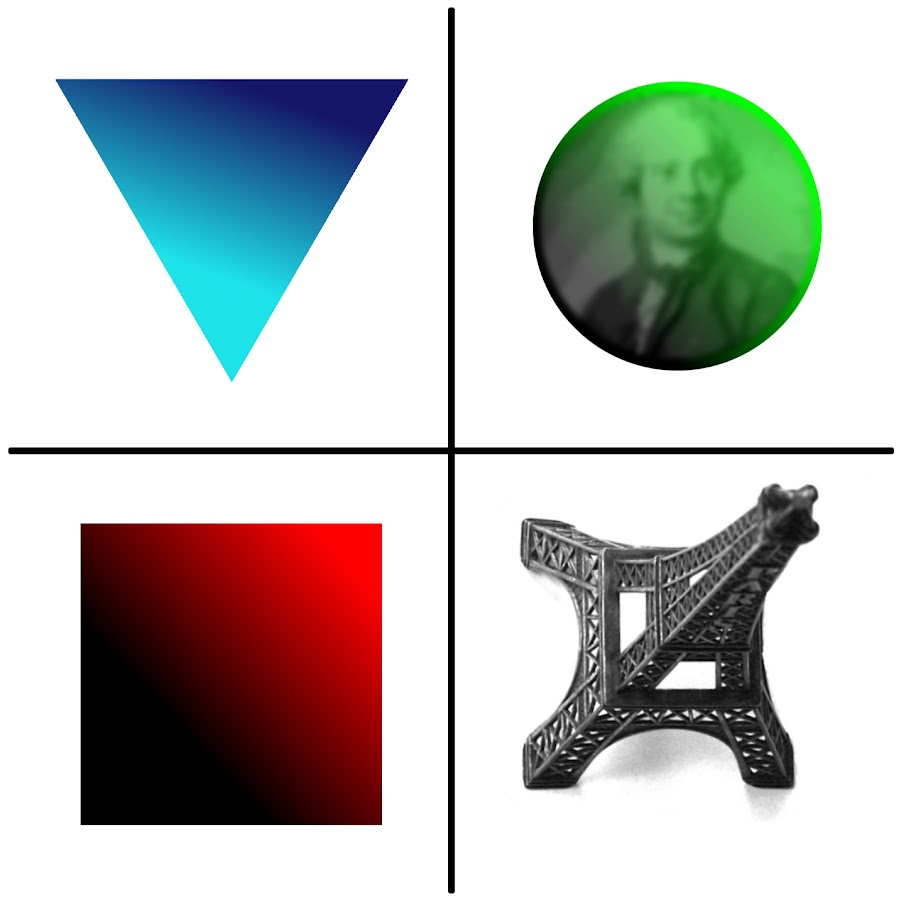
\includegraphics[height = 2cm]{Figures/logo_minimal_institut_jean_le_rond_dalembert.jpg}};

\begin{figure}[H]
    % \centering
    % \includegraphics[width = \textwidth]{Figures/image_represantation_schematique.png}
    % \caption{Representation schématique de l'environnement rude le quel les hydroliennes sont situe\autocite{title_fig}}
\end{figure}  
\thispagestyle{empty}

% \comment{
%     \vspace{1cm}
%     \begin{tabular}{m{6cm} m{5cm} m{3cm}}
%                      %\hline
%                      % after \\: \hline or \cline{col1-col2} \cline{col3-col4} ...
%                      %\bfseries{Report Type:} & Final & \\\\\\
%                      %\bfseries{Les étudiants} & Erdi ÇAN & \\\\\\
%                      %\bfseries{Thesis Director:} & Prof. Christian Enz & \dotfill{} \\\\\\
%                      \bfseries{Diercteur de recherche } & ... & %\dotfill{} \\\\\\
%                      %\bfseries{Date:} & \today  \\\\\\
%      %               \hline
%                    \end{tabular}%
% }
%\afterpage{\blankpage}

\newpage
\setcounter{page}{1}
\pagestyle{fancy}
\fancyhead{} % Clear all header fields
\setlength{\headheight}{24pt}
%\fancyhead[LE,RO]{\thepage} %
\fancyhead[CE,CO]{\HeaderDeReapport} %
\fancyfoot{} % Clear all footer fields
\fancyfoot[RE,LO]{\thepage}
%\fancyfoot[RE,LO]{\textit{\copyright A. Mangla}} %
%\fancyfoot[LE,RO]{\textit{%\today}} %
% \afterpage{\blankpage}


\pagenumbering{roman}
\section*{Résumé}{
}
\section*{Abstract}{
}
% \newpage
\section*{Remerciements}{
}
%\newpage

\tableofcontents
% \newpage
\listoffigures
\listoftables
%\newpage

\section*{Nomenclature}{
\begin{table}[H]
    % \centering
    % \caption{Values for blade and turbine thrust for each studied configuration.}
    \begin{tabular}{l c c} % ccc cccc cccc cccc   
        \toprule
        Symbole & Signification & Valeur \\
        \midrule
        $\bm{x}$ & Design variables TODO& \\
        $f(\bm{x})$ & Objective function & \\
        $g(\bm{x})$ & Inequality constraints TODO& \\
        $h(\bm{x})$ & Equality constraints TODO& \\
        \bottomrule
    \end{tabular}
\end{table}
      
}

\newpage

\section*{Premier mots des autheurs}

TODO premier mots ce que on a fait et les difficultes vite fait plutot pour dire nos ameliorations en math etc...

Dans ce rapport on utilise pas mal de references a notre anexe pour les bases et les definitions fondamentales utilise plusieur fois pour venir facilement en ariere nous conseillons de utiliser alt + left arrow pour revenir en ariene dans windows et linux et cmd + [ dans Mac OS X. Ou regarde le racourcis pour votre viever de pdf pour faciliter le retour. Si il y a un seul lien normalement on a essaye de mettre des references de retiur mais le premier est plus conseille.


\newpage    
\pagenumbering{arabic}

\chapter{Introduction}
\section{Introduction}
Lobjectid de loptimisation avec les enjeux et les avantages et pourquoi ca peut etre utile
\subsection{Optimisation}
Optimisation et les difficultes de l'optimisation car on peux faire une seul propriete l'optimal et si on a plusieurs parametres on a besoin de faire des compromis entre eux. Mais cela ne empeche pas de trouver le optimal de plusieurs couple. 
\begin{figure}[H]
    \centering
    \includegraphics[width = 0.8\textwidth]{example-image}
    \caption{Figure des valeur optimale de trainee et du lift}
\end{figure}

L'objective est de minimiser $f(x)$ (function objective) subject a $g(x)<0$ (constraints) et  $h(x)=0$ 
Mais comment on definit ces fonctions est que cest seulement que on essaye de minimiser la masse sans contrainte alors on a plus de objet car plus de pbjet veut dire que on aurait pas de masse et donc cest l'optimale. Pour cela le choix de fonction objective et des contraintes est tres importante. 

Procedure d'optimisation: on itere et ameliore le design jusque a la simulation converge. 

\chapter{Methods d'optimisation}

Les methodes de optimisation peut se partager en deux sous parties en premier methodes de optimisation avec gradient({\textit{gradient-based}}) et sans gradient ({\textit{gradient-based}}) et dans chaqun de ces categories on peux evoir des problemes de optimisation avec et sans contraintes.
TODO 
\begin{itemize}
    \item Advantages and disadvantages of each of them 
    \item differences 
    \item similarites
\end{itemize}

Algorithme d'optimisation sans contrainte 

Soit $F:\mathbb{R}^d \rightarrow \mathbb{R}$. On suppose qu'il $\exists  x^* \in \mathbb{R}^d$ tel que $F(x^*) = \inf_{x \in \mathbb{R}^d} F(x)$

On cherche a calculer $x^*$

TODO expliquer les methodes dans le diapo 28 de la presentation MIT $16.810_L0_Optimisation$

TODO pas sur de ici si il faut detailler cela ???

Il existe plusieurs classes de methodes:
\begin{itemize}
    \item  Méthodes de descente: consiste à construire une suite minimisante, c'est à dire $(x_k)_{k\in N}$ telle que 
    $$ F(x_{k+1}) \leq F(x_k) $$
    $$x_k \rightarrow x^* $$
    
    \item Méthodes basées sur l'équation d'Euler qui consiste à chercher une solution de l'équation $\nabla F(x) = 0$. Ces méthodes nécessitent donc que $F$ soit dérivable
\end{itemize} 
\section{Heuristic methods}
\section{Methodes base sur des gradients} \label{grad_methods}
Les methodes bases sur les gradients consiste a utiliser le gradient pour se diriger vers ou la fonction decroit et pour en suite trouver un minimum locale. Le deroulement de cela se passe en faisant l'algoritme suivant:
\begin{algorithm}[H]
    \begin{algorithmic}
        \State Initialisation de notre point de depart initale. $x_0 \in \mathbb{R}^d$
        \ForAll {$k$}
            \State Choisir une direction de descente $h_k$ de $F$ au point $x_k$
            \State Choisir un pas $t_k > 0$
            \If{$\nabla F (x_k) = 0$}
                \State \textbf{break} (On arette la boucle car on a trouve notre minimum locale)
            \EndIf
            \State $x_{k+1} = x_k + t_k h_k$
        \EndFor   
    \end{algorithmic}
    \caption{Algorithme de decente generic} % TODO Meilleeur caption
\end{algorithm}


% TODO comment l'exprimer nous meme ou autre alternative
\begin{lemma}[meilleure direction de descente locale] 
Soit $x \in \mathbb{R}^d $ telle que $\nabla F(x) \neq 0$. $h \in \mathbb{R}^d$ est une direction de descente si et seulement si $\langle \nabla F(x), h \rangle < 0$. En particulier, $h_{\nabla} : = -\frac{\nabla F(x)}{\lVert \nabla F(x) \rVert}$ est la meilleure direction de descente.
\end{lemma}


\subsection{Optimisation sans contrainte}

Soit $F:\mathbb{R}^d \rightarrow \mathbb{R}$. On suppose qu'il $\exists  x^* \in \mathbb{R}^d$ tel que $F(x^*) = \inf_{x \in \mathbb{R}^d} F(x)$

On cherche a calculer $x^*$

% Petit rappell: La heissienne de la fonction $F(\bm{x})$ est note $H_F(\bm x)$ avec $H_F(\bm x)\in \mathcal{M}_d(\mathbb{R})$


\subsection{Methode du gradient a pas constant}
La methode du gradient a pas constant coniste a prendre un point et se deplacer dans la direction contraire du gradient avec un pas consant choisi. La raison la quelle on prends la direction inverse du gradient est que le gradient donne la direction vers ou la fonction croit et nous on veut trouver le minimum. C'ette methode de descente prends un pas constant avec un pas $t_k = \tau > 0$, et une direction de descente $ h_k = - \nabla F(x_k)$. Donc notre formule diteration deviens: 

\[x_{k+1} = x_k - \tau \nabla F(x_k)\]

\begin{table}[H]
    \begin{tabularx}{\linewidth}{>{\parskip1ex}X@{\kern4\tabcolsep}>{\parskip1ex}X}
    \toprule
    \hfil\bfseries Avantages
    &
    \hfil\bfseries Desavantages
    \\\cmidrule(r{3\tabcolsep}){1-1}\cmidrule(l{-\tabcolsep}){2-2}
    %% PROS, seperated by empty line or \par
    Pas nescesaire de connaitre $F$ seulement $\nabla F$ suffit\par
    Pas besoin de iterer pour trouver un pas optimal\par
    &
    %% CONS, seperated by empty line or \par
    Le pas ces' possible que ca ne soit pas optimale\par
    \\\bottomrule
    \end{tabularx}
    \caption{Pros and cons gradient simple}
\end{table}

\begin{figure}[H]
    \centering
    \includegraphics[width = 0.8\textwidth]{example-image}
    \caption{Figure des iterations avec grad simple en 2D et 3D}
\end{figure}

\begin{figure}[H]
    \centering
    \includegraphics[width = 0.8\textwidth]{example-image}
    \caption{Figure du pas optimale droite avec une discretisation elevee gauche discretisation basse}
    \label{fig_optimal_pas_graphe_discretisations}
\end{figure}

\begin{figure}[H]
    \centering
    \includegraphics[width = 0.8\textwidth]{example-image}
    \caption{On choissisant le pas optimale pour avoir le moins de iteration comme vu dans la figure \ref{fig_optimal_pas_graphe_discretisations} le nombre diteration pour chaque point.}
\end{figure}

\subsection{Methode du gradient a pas quasi-optimale}
Dans ces methodes on trouve des pas quasi optimales pour aprocher au minimum avec moins de iterations.
\subsubsection{Regle d'Armijo}
\subsubsection{Regle de Wolfe}

\subsection{Methode du gradient a pas optimale}
Cette methode essaye de trouver la direction en prennant a la direction orthogonale de la direction precedente
\subsection{Adjoint}



\newpage
\thispagestyle{empty}
\nocite{*}
\addcontentsline{toc}{chapter}{Bibliographie}
\printbibliography[title = Bibliographie] % TODO \&{} Sitographie]

% \newpage

% \clearpage
% \pagenumbering{arabic}% resets `page` counter to 1
% \renewcommand*{\thepage}{A\arabic{page}}

% \twocolumn
\newpage
% https://tex.stackexchange.com/questions/174621/numbering-appendices-by-letter-instead-of-number

\appendix
\addcontentsline{toc}{chapter}{Annexes}
\chapter{TODO name of Annexes}
\renewcommand{\thefigure}{A\arabic{figure}}
\setcounter{figure}{0}
%\section{Annexes}
\setcounter{page}{1}
\renewcommand{\thepage}{A-\arabic{page}}

\section{NACA Naming}
mr samsam

\chapter{TODO name of Annexes}
\setcounter{page}{1}
\renewcommand{\thepage}{B-\arabic{page}}

\section{Bases mathematiques}
TODO comment faire les defintions pour que ca ne souit pas du plagiat????
\begin{definition}[$l^2$]
    
\end{definition}

\begin{definition}[Produit scalaire]
    Le produit scalaire dun $\mathbb{C}\mathrm{-espace}$ vectoriel $V$ est une application bilinear conjuge-symetrique. $$\langle ., . \rangle : V \times V \rightarrow \mathbb{C}$$

    telle que pour $ \forall x, y, z\in V$ et pour $\forall \lambda \in \mathbb{C}$,
    \begin{itemize}
        \item $\langle x, y \rangle = \overline{\langle y,x \rangle}$
        \item $\langle \lambda x, y \rangle = \lambda\langle x,y \rangle$
        \item $\langle x+y, z \rangle = \langle x,z \rangle + \langle y,z \rangle$
        \item $\langle x,x \rangle > 0 $ alors $x \neq 0 $
    \end{itemize}
    
    De cela on peut aussi definir l'espace préhilbertien qui est le pair $\langle V, \langle.,.\rangle \rangle$ ou $V$ est un $\mathbb{C}\mathrm{-espace}$ vectoriel et $\langle.,.\rangle$ est le produit scalaire sur $V$.
\end{definition}

TODO est que cela est vraie tout le temps ou dans les espaces fini pu $\mathbb{C}^\mathbb{N}$ Car si cest pas toujoursle cas TODO definir en espace infini

Si $x, y \in \mathbb{C}^n $ alors,
$$\langle x,y \rangle = \sum_{i=1}^{n} x_i \overline{y_i}$$
ou $x = (x_1, \ldots, x_n), y = (y_1, \ldots, y_n)$ et $\overline{y_i}$ est le conjuge complexe de $y_i$.  \newline (Petit rappel: si $z \in \mathbb{C} \Rightarrow \overline{z} = \mathrm{Re}(z) - \mathrm{Im}(z) $)

TODO je suis pas sur si cet defini seulement si x et y sont de mem dimension ou pas 
\begin{definition}[Espace dual]
    
\end{definition}



\begin{definition}[Espace d'Hilbert]

\end{definition}


% En faite l'adjoint est aussi une methode de gradient mais une methode moins mainstream et diifenente de ma lemhode du gradient parle dans \ref{grad_methods}. Pour cela une differente section a ete dedie.
% \input{annexe.tex}
TODO Est que il ya  des methodes pour trouver le minimum globale sans parcourir toute la fonction dans un temps fini ou notre meilleur choix est de faire une recherche aleatoire de decente et a la fin on a la posibilite de tomber dans un minimum globale?

\end{document}